\section{Lectures and Tutorials}
This section will depict a walk through for both the lectures and tutorials for each subsection.

\subsection{Overview Page}
The lectures and tutorials components are accessible from the side page of the course page. This will then render to users the overview page for either the lectures or tutorials component. Additionally, there will be a unique lectures and tutorials component for each different course.

\subsubsection{Purpose}
The purpose of the overview page is to display to users the existing weeks for either the lectures or tutorials component.

\subsubsection{What Was Implemented}
The overview page for the lectures and tutorials component is implemented via a list in chronological order of weeks to aid in readability of the component. Also, there is a panel for lecture/tutorial videos which display the external link to the videos.

\begin{figure}[h!]
    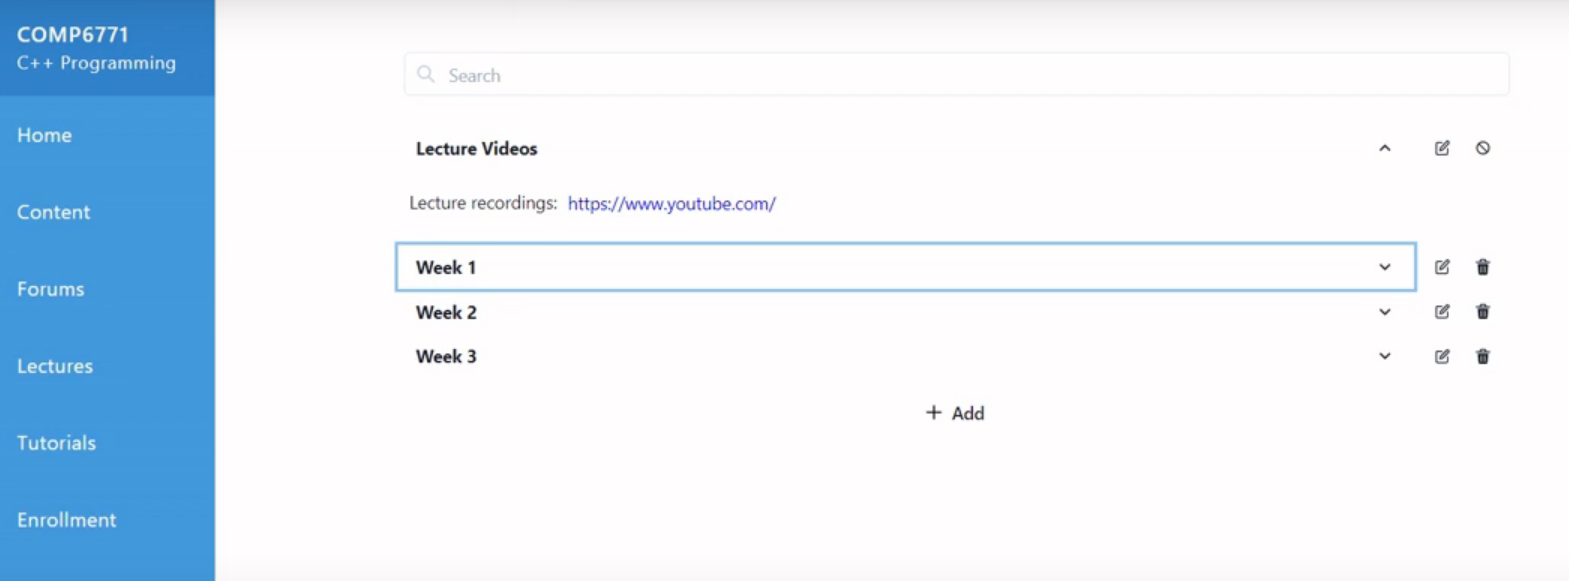
\includegraphics[scale=0.3]{lat-sidebar-lectures.png}
    \centering
    \caption{Lectures Page}
\end{figure}

\begin{figure}[h!]
    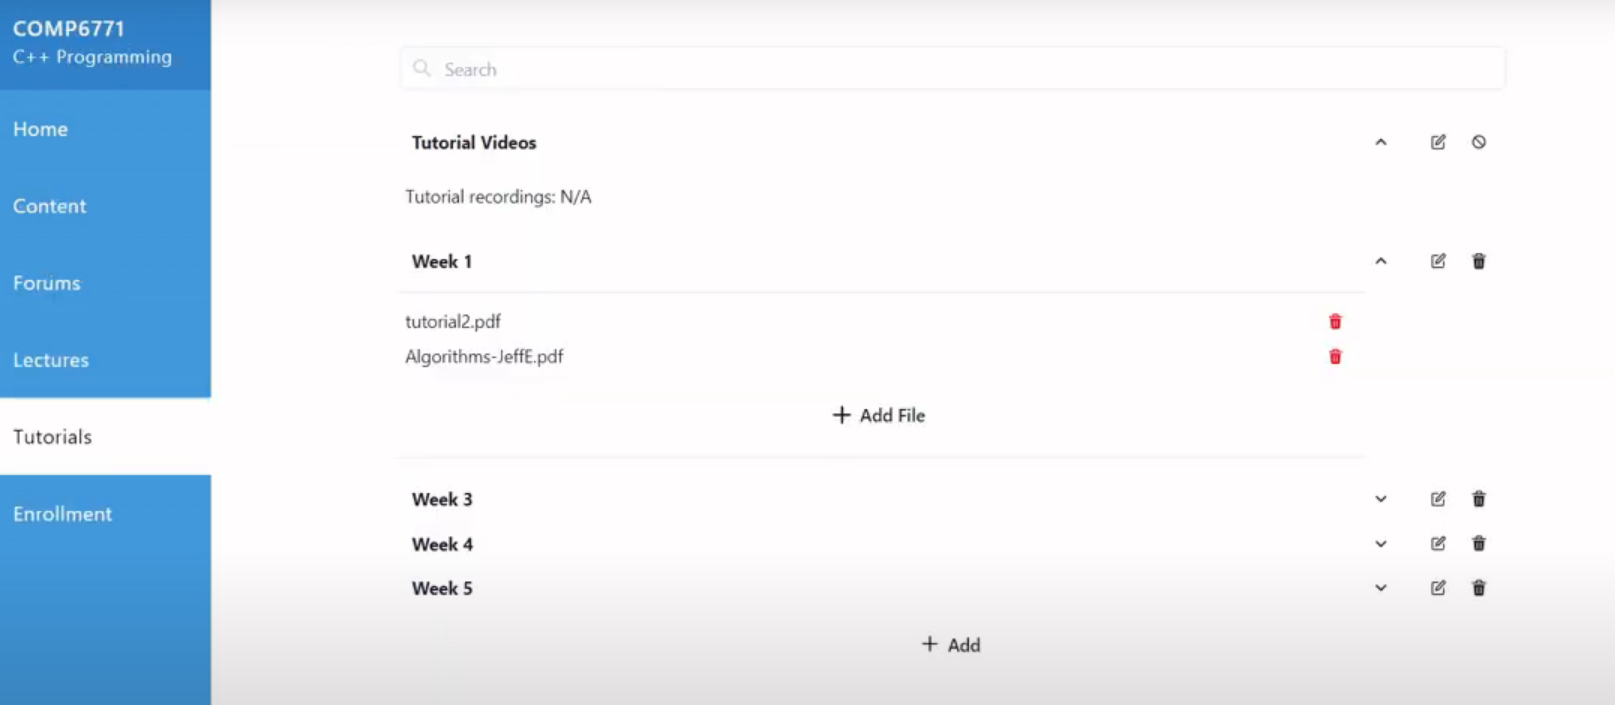
\includegraphics[scale=0.3]{images/lat-sidebar-tutorials.png}
    \centering
    \caption{Tutorials Page}
\end{figure}

\subsubsection{How It Was Implemented}
This component was implemented using the frontend tech stack. The component renders the lectures/tutorials and their corresponding files to the frontend using API calls to the backend.

\subsubsection{Considerations}
As there is a possibility of admin users creating wrong weeks, there is a functionality to edit the weeks to the users discretion. Additionally, if an admin user were to create an existing week with new uploaded files, the files would be added to the relevant week instead of creating a duplicate week. Also, the inclusion of trash and edit icons help infer their functionalities to users.

\subsection{Video Links}
The user is able to clear an existing video link to recordings or streams by clicking the related clear button. Additionally, users can also edit and add another link to their external video platform.

\subsubsection{Purpose}
The purpose of the video links feature is to allow admins to update the video links and for students to access their lecture/tutorial recordings or attend the lectures/tutorials.

\subsubsection{What Was Implemented}
There is a panel in the overview page that depicts the relevant lecture/tutorial video links. In this panel, there is a hyperlink to the admins chosen video hosting site. For instance, the admin may choose to set the link to a YouTube link. Also, there is an edit button that allows admins to edit the link to their liking and a clear button which allows admins to clear the link and set it to N/A.

\begin{figure}[h!]
    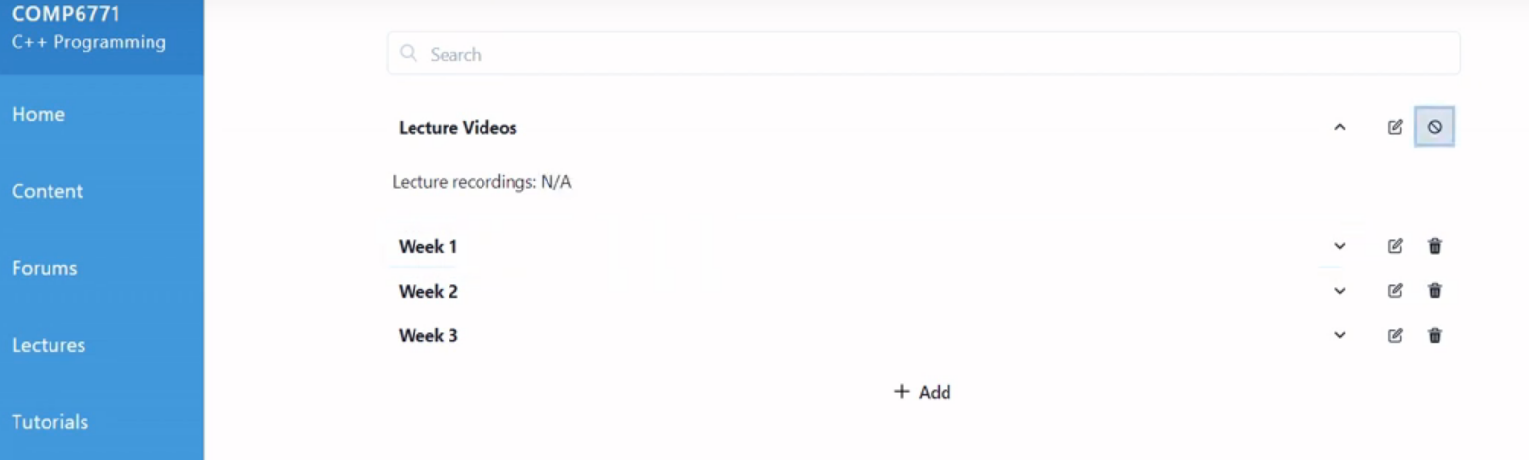
\includegraphics[scale=0.3]{images/lat-lectures-clear-link.png}
    \centering
    \caption{Clearing a video link}
\end{figure}

\begin{figure}[h!]
    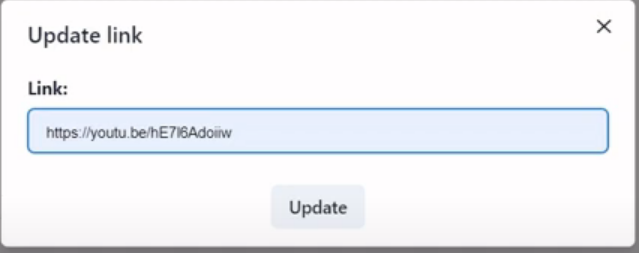
\includegraphics[scale=0.3]{images/lat-update-link.png}
    \centering
    \caption{Adding a new video link}
\end{figure}

\subsubsection{How It Was Implemented}
This component was implemented using an API from the backend that retrieves the current video link and renders it into the panel. Also, this component uses APIs to edit and delete the link to the admins discretion.

\subsubsection{Considerations}
There is a potential for admin users to enter an invalid link, which the component would then notify the user that there was an invalid link inputted. As a result, this ensures that admin users correctly input links to their lecture/tutorial videos. Moreover, admins may also clear and set the link to N/A to ensure that student users are aware that there are no lecture/tutorial videos available. Also, users whom are students are unable to edit the video links but are able to click on the links themselves.

\subsection{Weeks}
The weeks sections will include: adding weeks, deleting weeks and editing weeks for the lectures and tutorials feature.

\subsubsection{Purpose}
The purpose of the weeks feature is to allow users to distinguish between weeks in a tutorials/lectures component. This also allows users to determine the relevant course materials for their corresponding weeks of the course also.

\subsubsection{What Was Implemented}
In the overview page, there are panels present that indicate the weeks present in the relevant lecture/tutorials of the course. A user may click on the relevant weeks to reveal files corresponding to the week.

At the bottom, there is an addition button that infers to users that it adds a week to the table. This would open a modal which includes a week and file inputs. 

\begin{figure}[h!]
    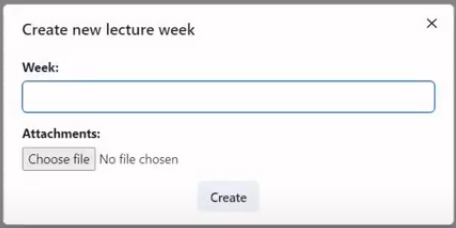
\includegraphics[scale=0.3]{images/lat-add-week.png}
    \centering
    \caption{Adding a week}
\end{figure}

There exists bin icons to the right of each week to indicate deleting for each week. 

\begin{figure}[h!]
    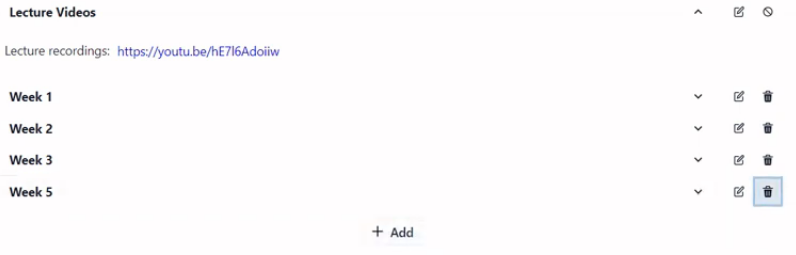
\includegraphics[scale=0.3]{images/lat-delete-week.png}
    \centering
    \caption{Deleting a week}
\end{figure}

Also, on the right side of each week would also include an editing icon which indicates modifying the week number. Once clicked, this reveals a modal which allows admin users to input a week number to update with.

\begin{figure}[h!]
    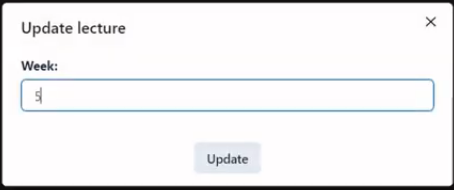
\includegraphics[scale=0.3]{images/lat-update-week.png}
    \centering
    \caption{Editing a week}
\end{figure}

\subsubsection{How It Was Implemented}
The component was implemented using APIs from the backend that involve retrieving the weeks of a lecture/tutorials for the course, deleting weeks, adding and editing weeks for the lectures/tutorials. Specifying either lectures or tutorials and inputting the course code in the backend would allow for a request that returns the weeks. Also, deleting and editing a week is possible through an input specifying the ID attribute and sending it to the API. Moreover, in order to add a week the admin user must provide the week number and if desired a file input. 

\subsubsection{Considerations}
The adding, editing and deleting weeks functions are only available to admin users, whereas student users are only able to view the weeks. Also, admins may wish to edit weeks that are already created to suit their needs. Additionally, the weeks are sorted in chronological order to aid in readability for users. Also, when an admin user creates a new week where the week number is 1 then that week would appear near the top once rendered.

\subsection{Files}
The files section includes: adding files, deleting files and downloading files for the lectures and tutorials component.

\subsubsection{Purpose}
The purpose of the files functionality is to allow users to download relevant files, admin users to delete and upload new files to the lectures/tutorials component of the course. 

\subsubsection{What Was Implemented}
In the lectures and tutorials overview page, there are expandable panels which then reveal to users files that relevant to each week in the lectures/tutorials component. There is also an addition button with an add file description that infers users of its function. 

\begin{figure}[h!]
    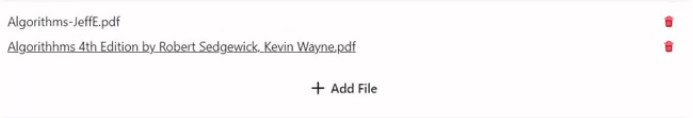
\includegraphics[scale=0.3]{images/lat-add-file.png}
    \centering
    \caption{Adding a file}
\end{figure}

There is a bin icon that is on the right side of the relevant file name or row in the panel which would infer to users that this would delete the file from the lectures/tutorials system for the relevant course.

\begin{figure}[h!]
    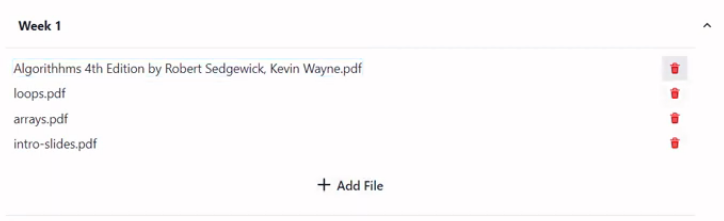
\includegraphics[scale=0.3]{images/lat-delete-file.png}
    \centering
    \caption{Deleting a file}
\end{figure}

The user is also able to download a file by clicking on the relevant file name or row in the panel.

\begin{figure}[h!]
    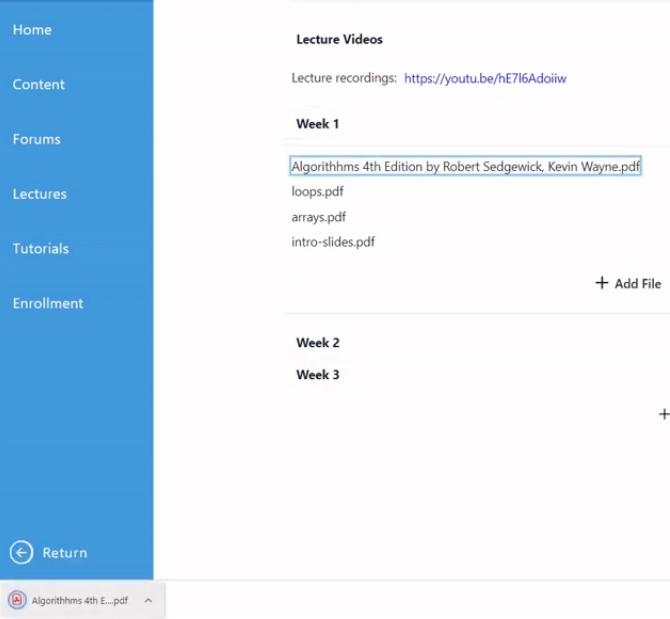
\includegraphics[scale=0.3]{images/lat-download-file.png}
    \centering
    \caption{Downloading a file}
\end{figure}

\subsubsection{How It Was Implemented}
The component was implemented using APIs from the backend that involve: posting new files to the server and deleting files from the backend. In the adding a file, there will be a file attached which is then used for a POST api which saves the file locally and the address is kept into a table in the database. Then when the user wants to download a file, the user simply clicks the link to the file which is a reference to the files physical location on the server. Also, in order to delete a file the user clicks the relevant bin icon for the item which then sends to the backend the ID of the item to remove from the server.

\subsubsection{Considerations}
There is a consideration where a user may also want to create a week and upload items simultaneously. This would add to efficiency of the feature. Additionally, adding a week that already exists with a file would then upload the file to the relevant week. This allows for admin users that may make mistakes in creating a week with files that already exist. Also, only admin users are able to add and delete files in the lectures/tutorials feature of the course.

\subsection{File Searching}
All users are able to search for a file in the lectures/tutorials sections by typing keywords that match to available files in the system.

\subsubsection{Purpose}
The purpose of the file searching feature is to allow users to quickly look for any files related to their inputs. For instance, a user may wish to see which files are PDFs in the lectures section of their course.

\subsubsection{What Was Implemented}
In the lectures or tutorials overview page, there is a search bar at the top that allows for users to input queries which then match to files in the lectures/tutorials system. When the user inputs a query, the overview page will then render a results table depicting all the file matches in relation to the search query.

\begin{figure}[h!]
    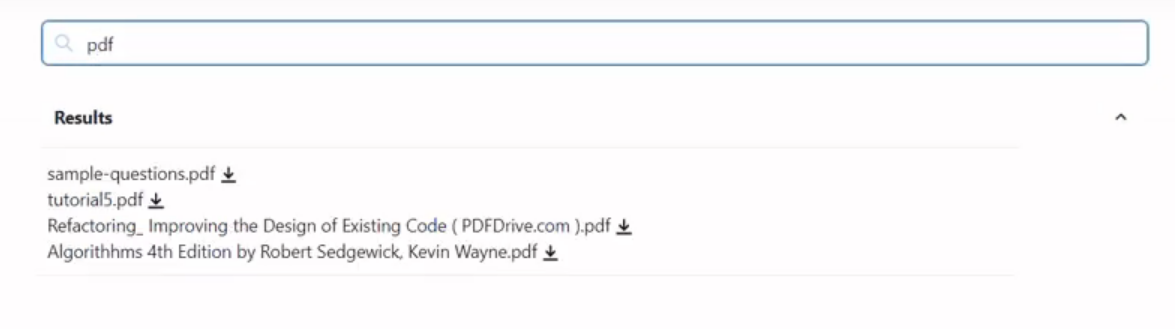
\includegraphics[scale=0.3]{images/lat-search.png}
    \centering
    \caption{Searching for a file}
\end{figure}

\subsubsection{How It Was Implemented}
The component was implemented using APIs from the backend that involve searching for a file either in the lectures or tutorials tables in the database. Also, implementing the search bar and its results were possible using ChakraUI and ReactJS. When the user enters an input search query, the query is sent to the backend which then searches for files that match that query and then output a list of files that have been matched to the frontend. Then the frontend takes this response and then renders it into the results table.

\subsubsection{Considerations}
There was a consideration for users who may wish to search via the type of file in the system such as PDF or doc. This allows for an extra parameter for searching available for all users. Additionally, in the future there will be an implementation where instead of submitting the search query, the files automatically filter based on keystrokes made by the user.